\section{Feature matrix} 
Finally, the evaluation results of three platforms are put together and incorporated into the feature matrix. The general structure of the matrix is showed in figure \ref{fig:featurematrix}.

\begin{figure}[h]
	\begin{adjustwidth}{-1.5cm}{}
	\centering
	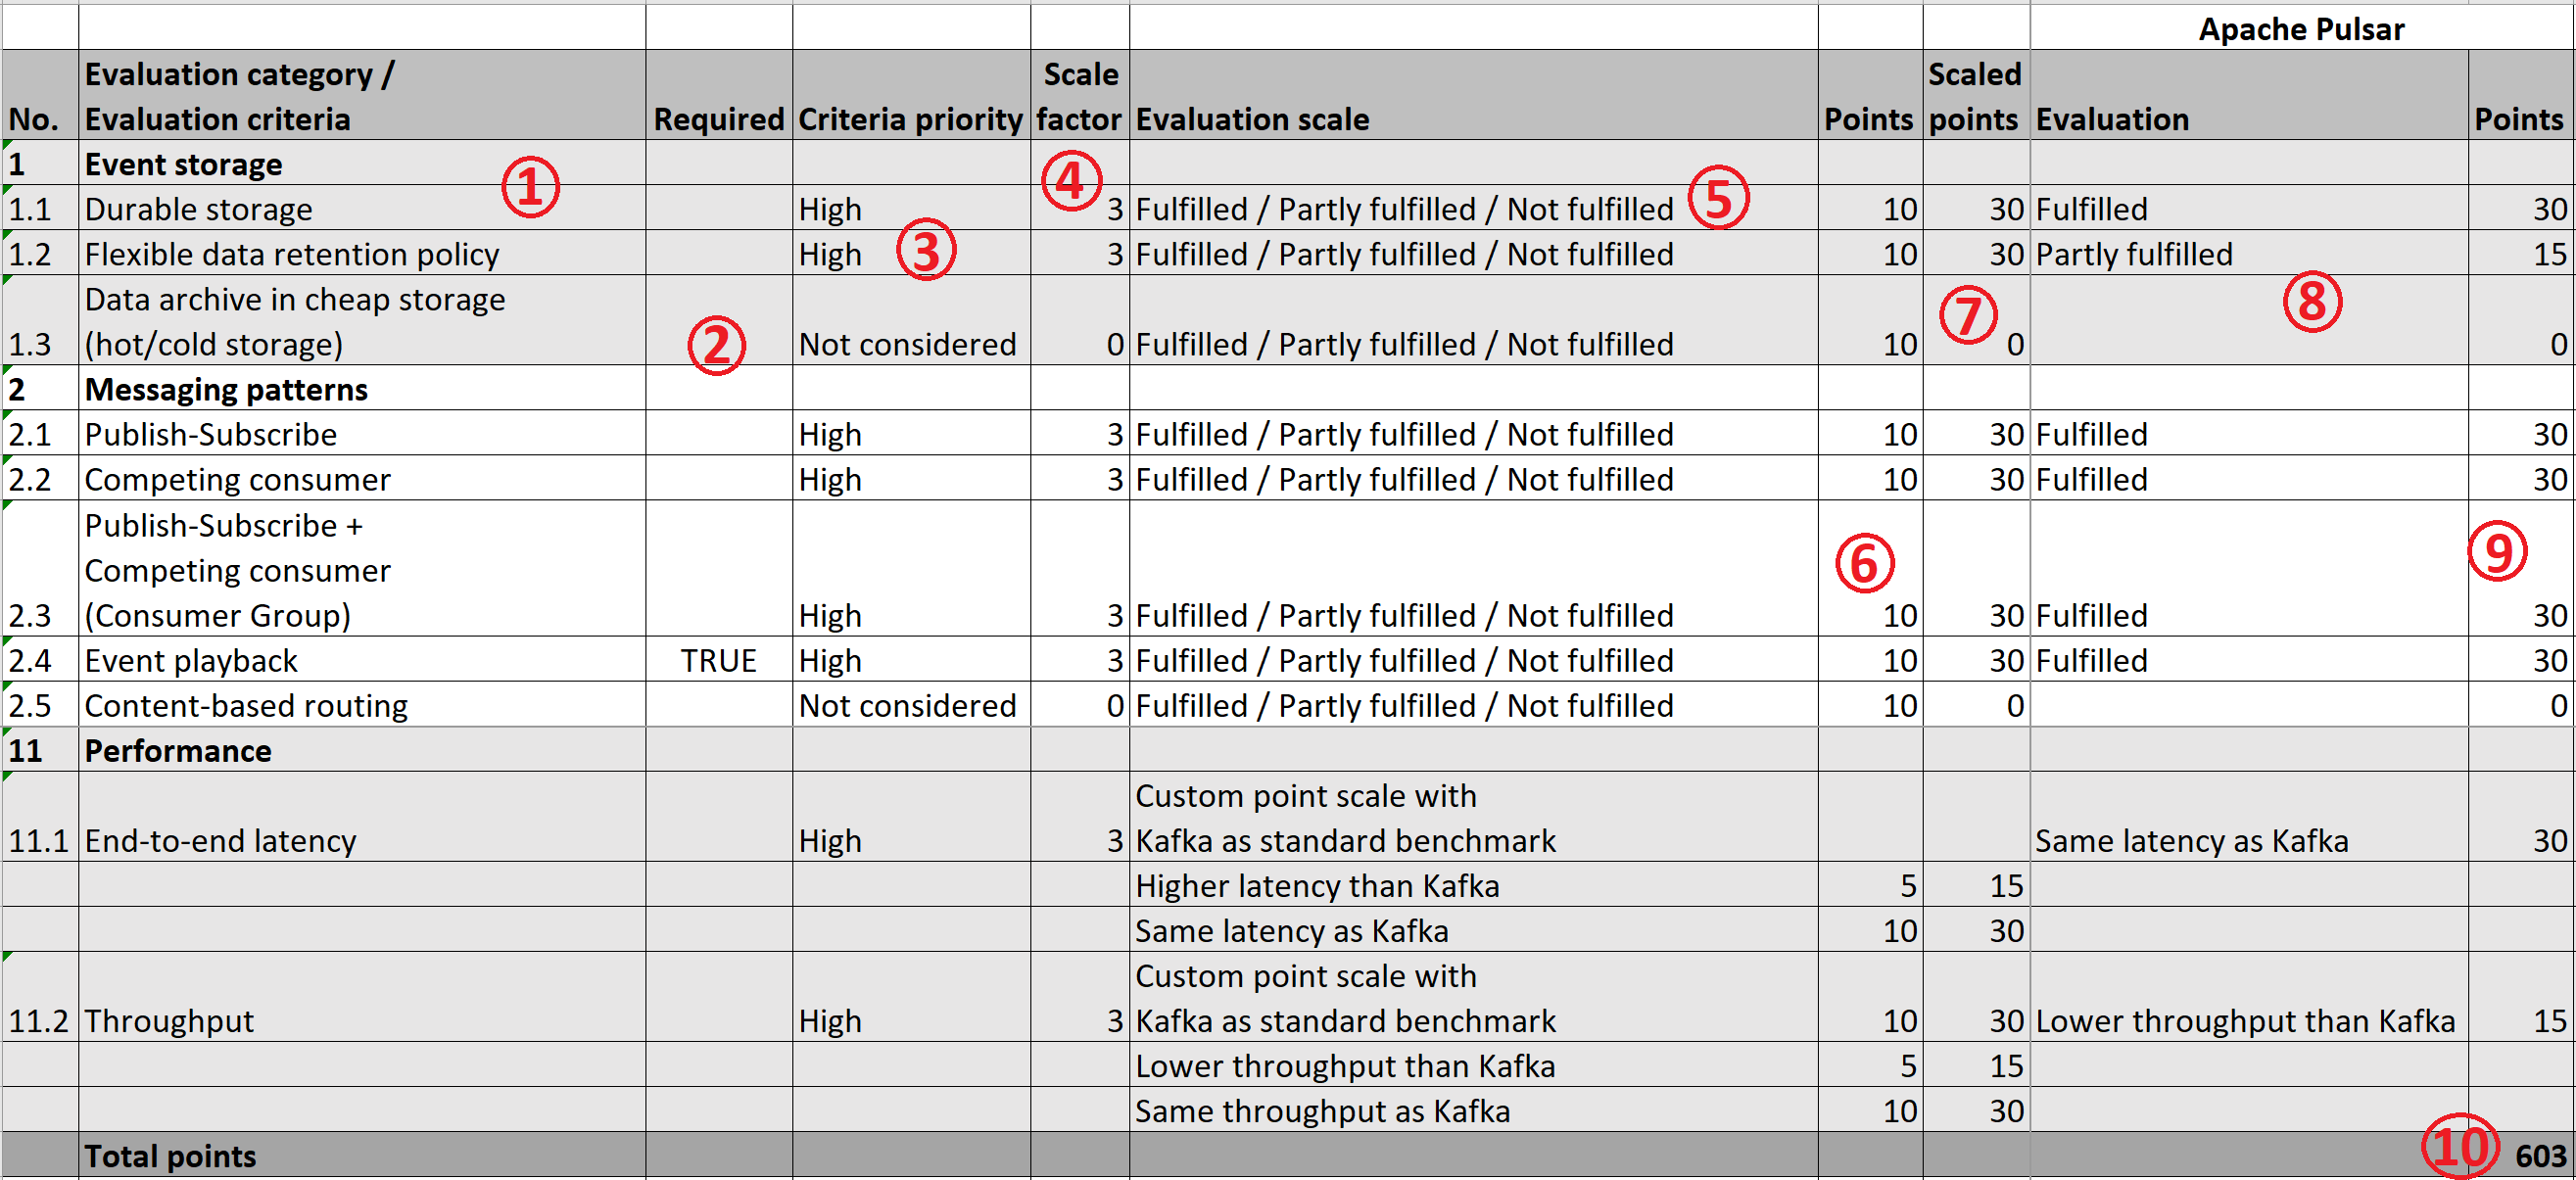
\includegraphics[width=18cm,height=4.5cm]{images/feature-matrix.png}
	\end{adjustwidth}
	\caption{General structure of the feature matrix.}
	\label{fig:featurematrix}
\end{figure}

In the matrix, users has the flexibility to choose different priority for each criterion. 